\localauthor{Thomas Kirz}

\subsection{Hochladen einer Revision}\label{subsec:sequenz-revision-hochladen}

Als Beispiel für einen Datenfluss wird ein in Abbildung \ref{fig:upload-revision-sequence} Sequenzdiagramm zu folgendem Hochladen betrachtet:
Ein angemeldeter Nutzer navigiert zur Seite einer eigenen Einreichung, für die eine Revision angefordert wurde.
Dort fügt er eine Revision, also ein neues Paper hinzu.

\begin{figure}[H]
    \centering
    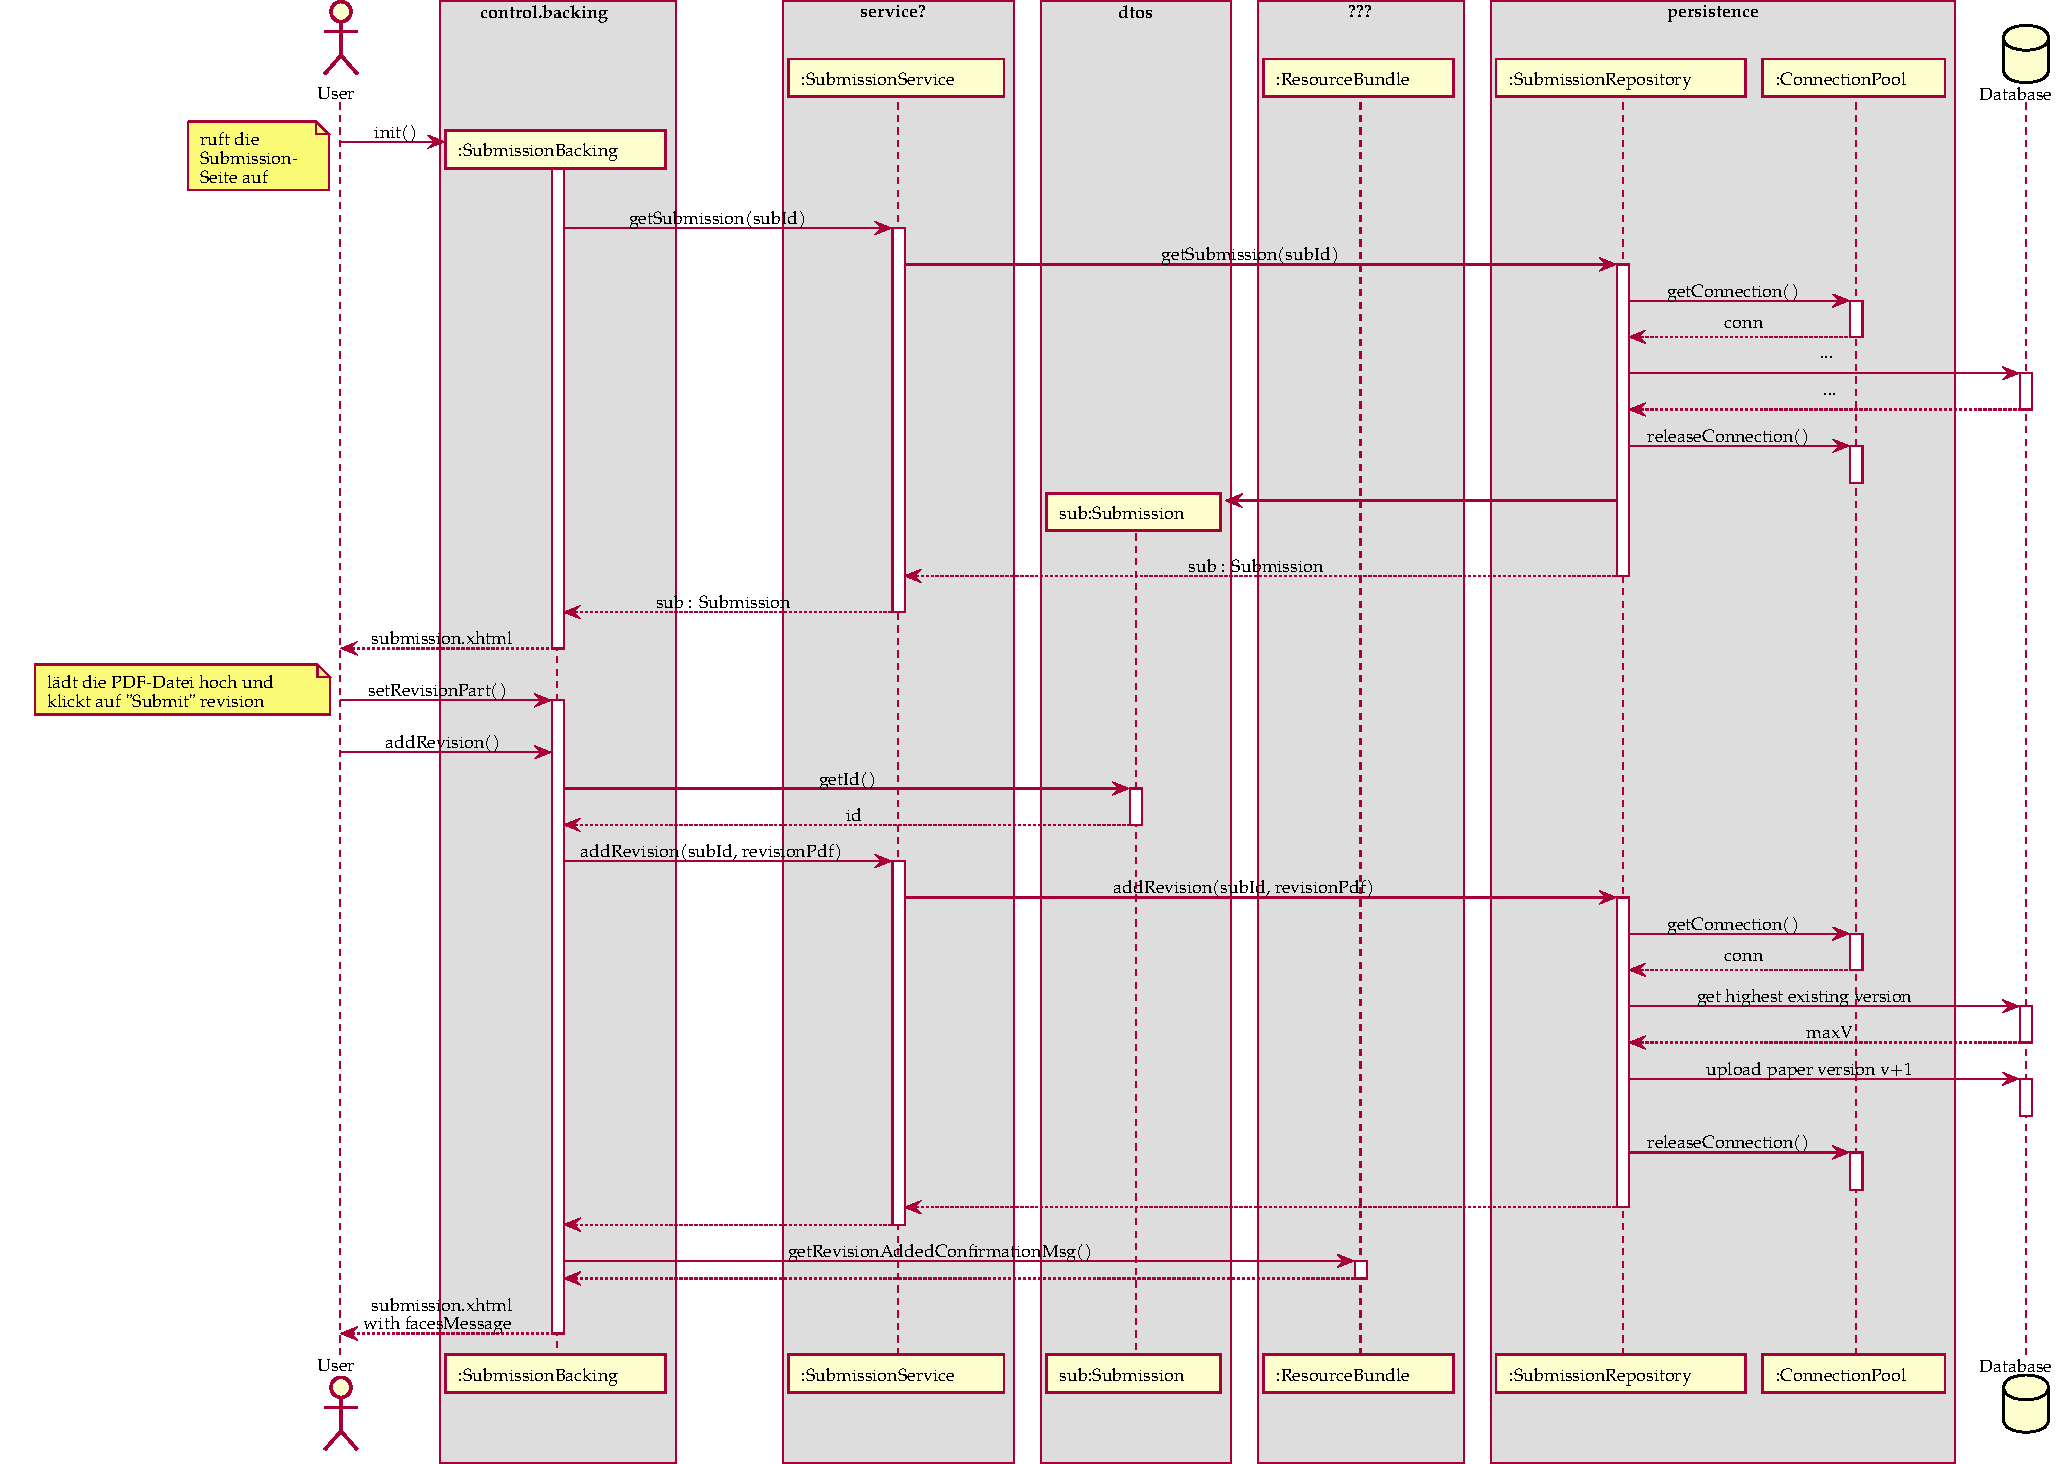
\includegraphics[width=0.8\textwidth]{graphics/upload_revision}
    \caption{Sequenzdiagramm zur Ablehnung einer Einreichung}
    \label{fig:upload-revision-sequence}
\end{figure}

\subsection{Ablehnung einer Einreichung}\label{subsec:sequenz-ablehnung}

Abbildung~\ref{fig:rejection-sequence} zeigt die Interaktionen zwischen den Klassen beim Ablehnen einer Einreichung, die Verbindung zum Datenbankserver schlägt aber fehl und die Einreichung kann nicht verändert werden.
Hier ruft ein Editor die Seite einer Einreichung auf und klickt auf den Button zum Ablehnen.
Beim Datenbankzugriff für die Aktualisierung des Status passiert ein Timeout.
Da dies ein fataler Fehler ist, wird der Nutzer mithilfe des ExceptionHandlers auf eine Fehlerseite weitergeleitet.

\begin{figure}[H]
    \centering
    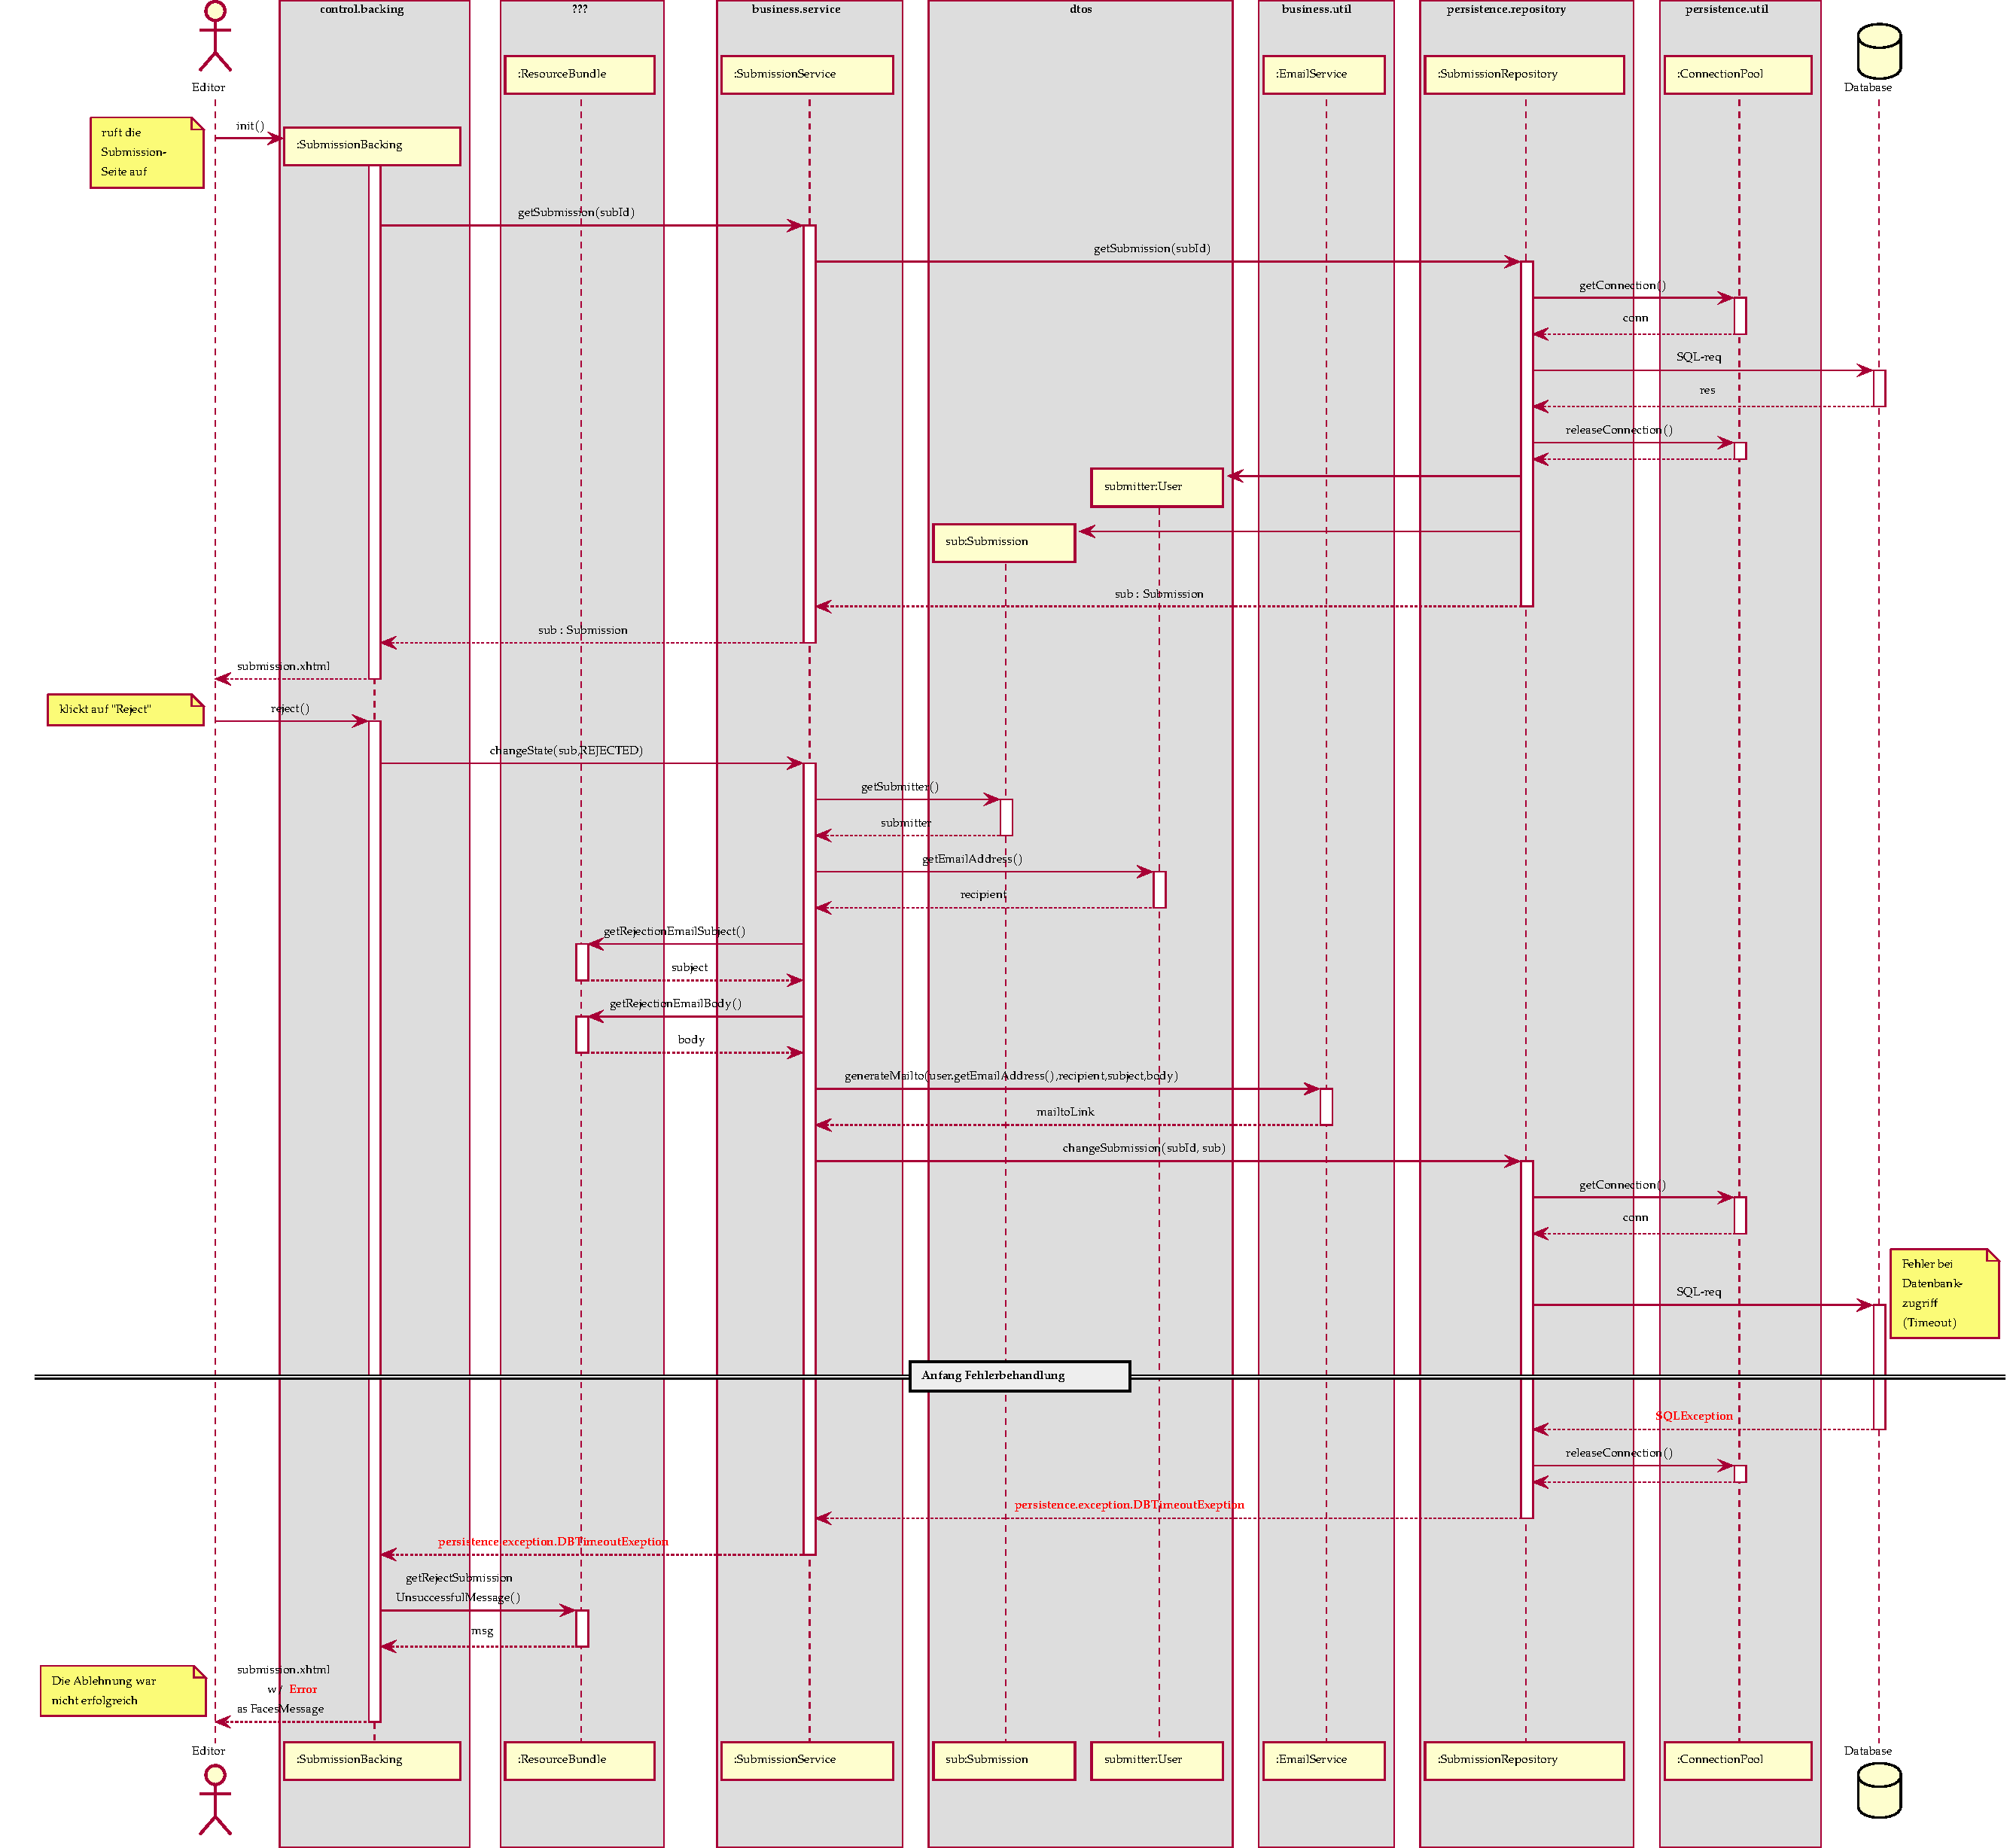
\includegraphics[width=0.8\textwidth]{graphics/reject_submission}
    \caption{Sequenzdiagramm zur Ablehnung einer Einreichung}
    \label{fig:rejection-sequence}
\end{figure}
